\documentclass[14pt]{beamer}
\usepackage{hyperref}
\usetheme{boxes}
\usecolortheme{dove}
\usepackage{txfonts}

\title{There And Back Again}
\subtitle{Databases At Uber}
\author{Evan Klitzke}
\date{October 4, 2016}

\begin{document}

\begin{frame}
  \titlepage
\end{frame}

\AtBeginSection[]
{
  \begin{frame}[plain]{Outline}
    \tableofcontents[currentsection]
  \end{frame}
}

\section{Background}

\begin{frame}{Uber Engineering Blog Post}
  \makebox[\textwidth]{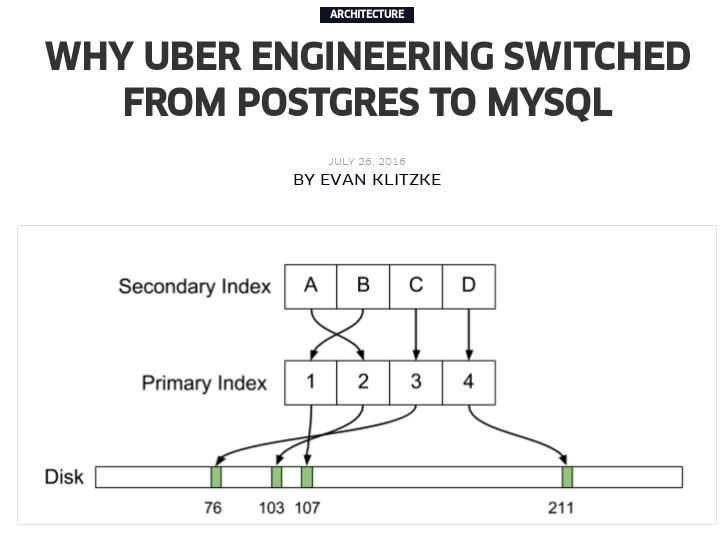
\includegraphics[scale=0.35]{blogpost.png}}
\end{frame}

\begin{frame}{Thanks Balaji}
  \makebox[\textwidth]{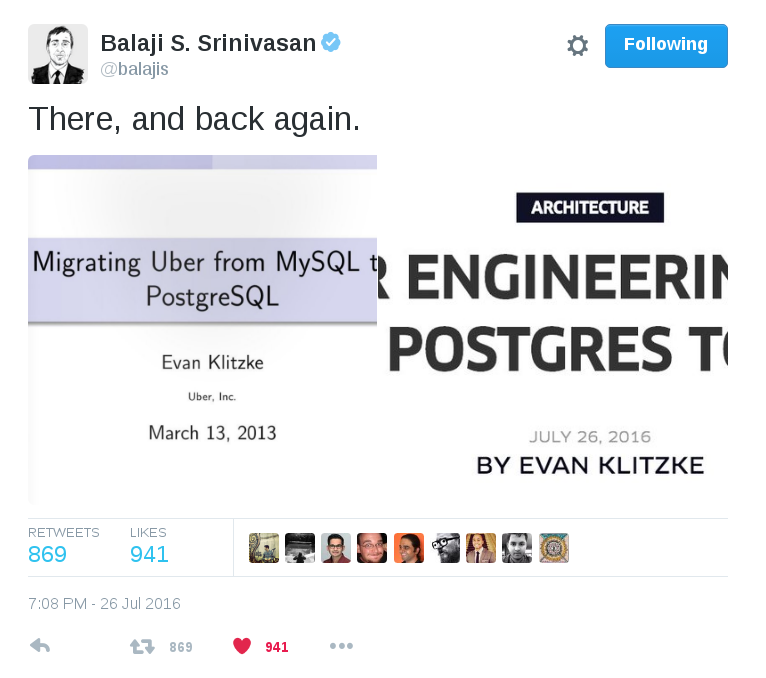
\includegraphics[scale=0.30]{balaji.png}}
\end{frame}

\section{MySQL To Postgres}

\begin{frame}{Company Background}
  When I joined in September, 2012:
  \begin{itemize}
    \item Company was about two years old
    \item About 30 engineers
    \item No DBA, only one person with an ops background
    \item I happened to be the person with more of a database background than
      anyone else, but I wasn't an DBA
  \end{itemize}
\end{frame}

\begin{frame}{Database Background}
  When I joined in September, 2012:
  \begin{itemize}
    \item Monolithic MySQL cluster
    \item One MySQL master, three or four slaves
    \item Examples of stored data: trips, user data, driver info, city data,
      fare structures, geofence information, toll data, etc.
    \item Database was $\sim500$ GB in size
    \item Bare metal hardware in a colocation facility; 15K SAS drives, lots of
      memory/CPU
  \end{itemize}
\end{frame}

\begin{frame}{Why We Wanted To Switch}
  Reasons:
  \begin{itemize}
  \item Technical
  \item Non-technical
    \end{itemize}
\end{frame}

\begin{frame}{PostGIS}
  Uber is an incredibly geo-centric company, and we had lots of geo data in the
  database:
  \begin{itemize}
    \item Trip points
    \item Geofence definitions
    \item Toll/tunnel definitions
    \item Etc.
  \end{itemize}
  There were also lots of ideas on new features that would heavily use
  geospatial information in the app, and it was thought that PostGIS would help.
\end{frame}

\begin{frame}{Online Schema Changes}
  We were making a \textbf{lot} of schema changes.
  \newline
  \newline
  For better or worse, there was a strong culture of shipping code quickly,
  sometimes without proper design. This led to a rapidly evolving schema and
  rapidly evolving index requirements.
\end{frame}

\begin{frame}{Hacker News Hype Cycle}
  MySQL is the database everyone loves to hate:
  \begin{itemize}
    \item Various poor default settings (esp. in older releases)
    \item Sordid history of replication bugs
    \item Somehow gets associated with PHP?
    \item Late to the game on ``sexy'' features like geospatial, JSON
      types, table inheritance, etc.
    \item Oracle is ``evil''
  \end{itemize}
\end{frame}

\begin{frame}{People Haven't Heard Of Postgres?}
  \makebox[\textwidth]{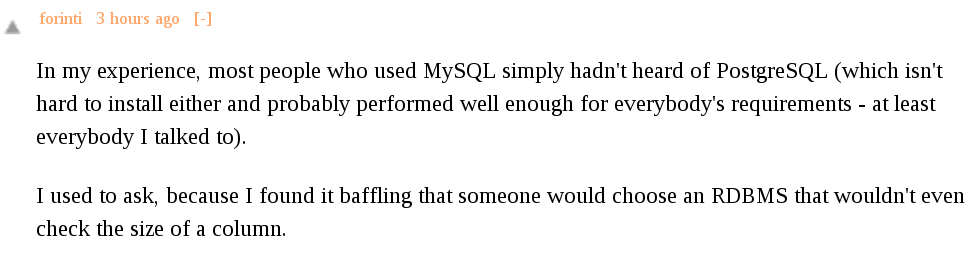
\includegraphics[scale=0.35]{never_heard.png}}
\end{frame}

\begin{frame}{MySQL Eats And Corrupts Data By Design}
  \makebox[\textwidth]{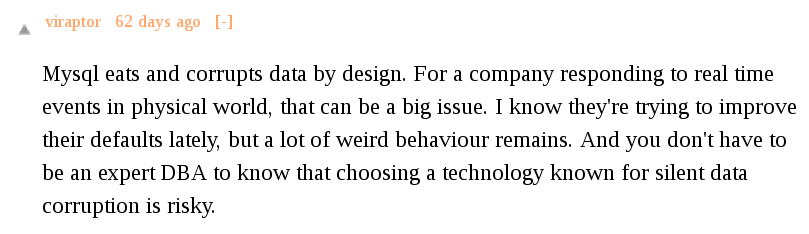
\includegraphics[scale=0.40]{corruption.png}}
\end{frame}

\begin{frame}{My Favorite HN Comment Ever}
  \makebox[\textwidth]{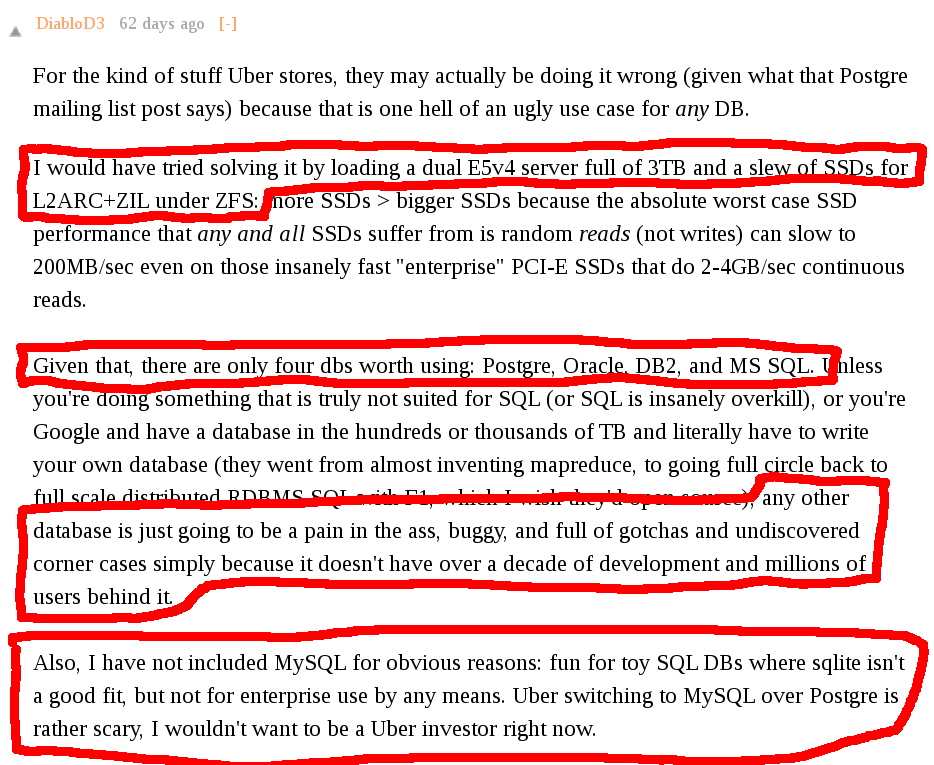
\includegraphics[scale=0.25]{favorite_comment_ever.png}}
\end{frame}

\begin{frame}{Hindsight Is 20/20}
  In retrospect, a lot of the motivation for moving to Postgres was fueled by
  this kind of hype.
  \newline
  \newline
  No one at Uber actually had experience running Postgres at
  scale and we didn't do realistic load testing before switching.
\end{frame}

\begin{frame}{Why I'm Telling You This}
  When you're moving quickly it's easy and tempting to take technical shortcuts
  and rely on hearsay. It happens to the best of us.
  \newline
  \newline
  It's incumbent on all of us, as engineers, to be objective, skeptical, and
  fact-driven.
  \newline
  \newline
  \href{https://www.youtube.com/watch?v=9vQaVIoEjOM}{Don't believe the hype.}
\end{frame}

\section{Connection Scalability}

\begin{frame}{Connection Scalability}
  From \texttt{wiki.postgresql.org},
  \href{https://wiki.postgresql.org/wiki/Number_Of_Database_Connections}{``Number
    Of Database Connections''}:
  \newline
  \newline
  ``A formula which has held up pretty well across a lot of benchmarks for years
  is that for optimal throughput the number of active connections should be
  somewhere near ((core\_count * 2) + effective\_spindle\_count). Core count
  should not include HT threads, even if hyperthreading is enabled.''

\end{frame}

\begin{frame}{Connection Scalability}
  From \texttt{wiki.postgresql.org},
  \href{https://wiki.postgresql.org/wiki/Tuning_Your_PostgreSQL_Server}{``Tuning
    Your PostgreSQL Server''}:
  \newline
  \newline
  ``Generally, PostgreSQL on good hardware can support a few hundred connections.''
\end{frame}

\begin{frame}{Milliseconds/Query}
  \makebox[\textwidth]{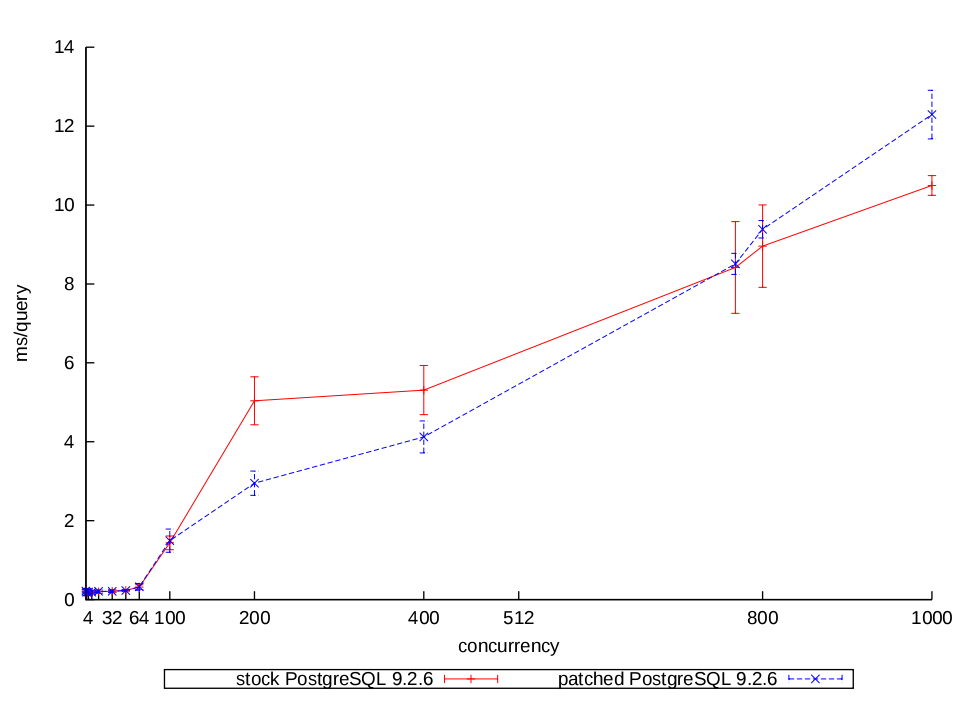
\includegraphics[scale=0.30]{ms_query.png}}
\end{frame}

\begin{frame}{QPS}
  \makebox[\textwidth]{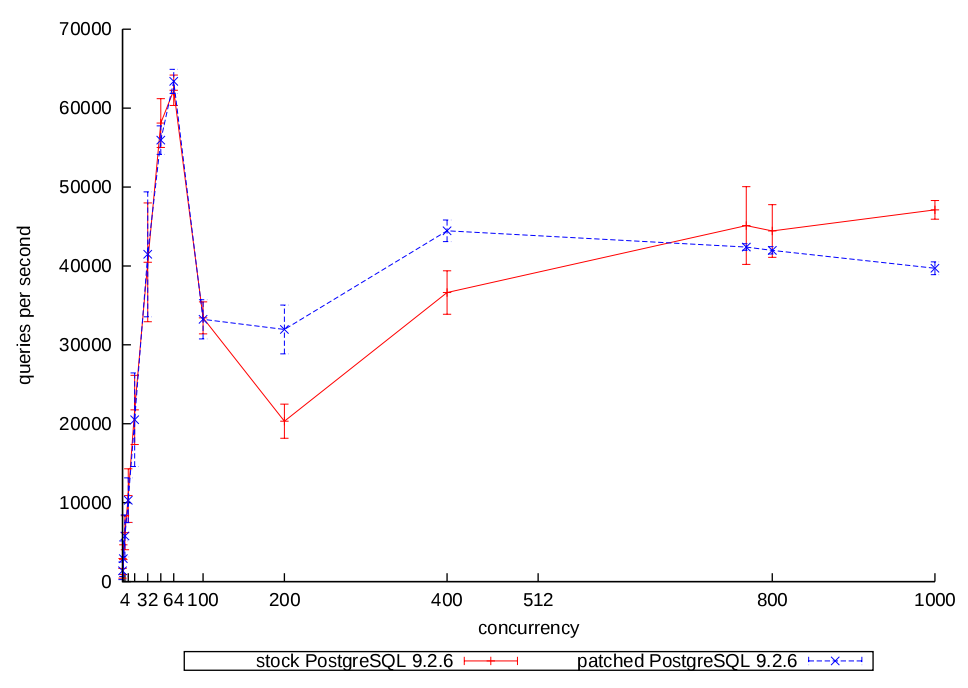
\includegraphics[scale=0.30]{qps.png}}
\end{frame}

\begin{frame}{A Real Uber Outage}
  This graph is from an outage in November, 2014:
  \newline
  \newline
  \makebox[\textwidth]{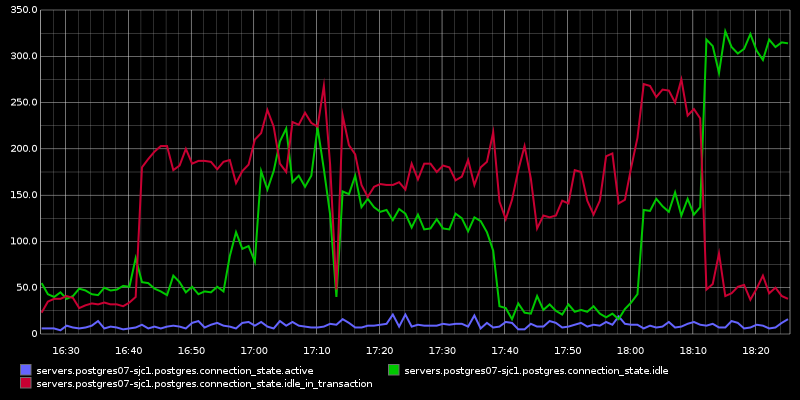
\includegraphics[scale=0.35]{outage.png}}
\end{frame}

\section{Write Amplification/Replication}

\begin{frame}{How Postgres Replication Works}
  Postgres maintains a write-ahead log (WAL) for crash recovery purposes. The
  WAL contents are very low-level, representing actual on-disk changes.
  \newline
  \newline
  Slaves stream WAL files from the master and apply them as if they're in
  crash-recovery.
\end{frame}

\begin{frame}{How Postgres Row Updates Work}
  Row ``tuples'' in Postgres are immutable.\footnote[1]{Except for ``heap-only
    tuples'' (HOT)}
  \newline
  \newline
  A tuple is updated by creating a new copy at a new location. Later the
  autovacuumer will reclaim old tuples.

\end{frame}

\begin{frame}{How Postgres Indexes Work}
  Index entries have a reference to the \texttt{ctid} of the row they index.
  \newline
  \newline
  \textbf{Pro:} Index lookups are very efficient!
  \newline
  \newline
  \textbf{Con:} All indexes must be updated when rows are updated, because the
  new row tuples will have new ctids.
\end{frame}

\begin{frame}{Replication Bandwidth}
  Guess what happened here (February, 2014):
  \newline
  \newline
  \makebox[\textwidth]{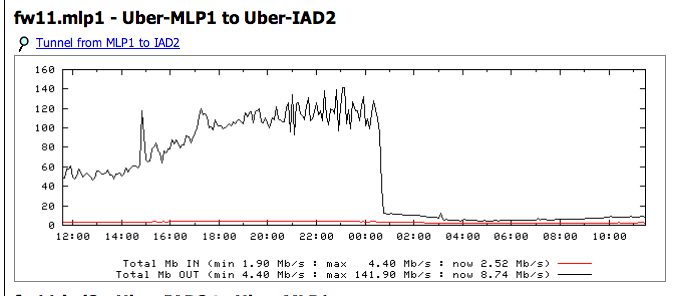
\includegraphics[scale=0.40]{bandwidth.png}}
\end{frame}

\begin{frame}{WARM}
  Postgres developers are working on this issue :-D
  \newline
  \newline
  \makebox[\textwidth]{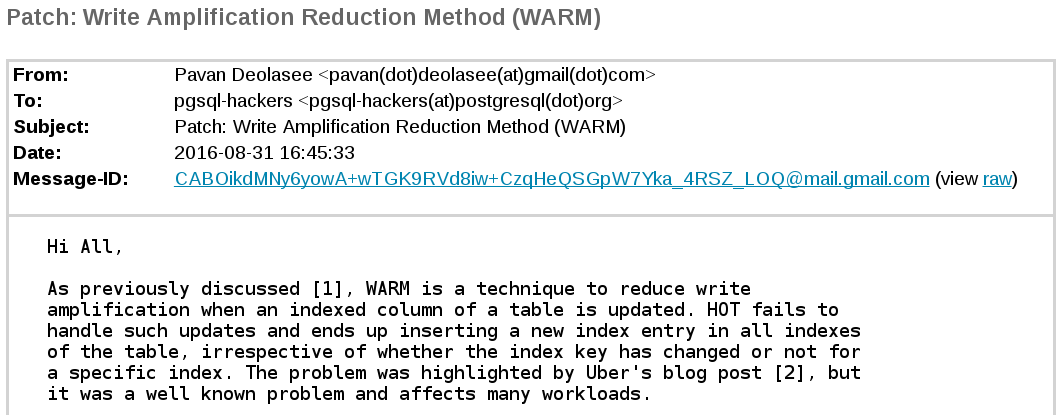
\includegraphics[scale=0.30]{warm.png}}
\end{frame}

\section{Miscellaneous Other Things}

\begin{frame}{Postgres Upgrades}
  How do you upgrade Postgres 9.2 to something newer?
\end{frame}

\begin{frame}{Buffer Pools vs. Kernel Page Cache}
  Reasons MySQL's ``buffer pool'' design is great:
  \begin{itemize}
  \item More efficient
    \item Not tied to on-disk format
  \item Fewer context switches
  \item Allows more efficient buffered writes
  \item Cool statistics, e.g. hit rate
  \end{itemize}
\end{frame}

\section{Databases at Uber Today}

\begin{frame}{Databases at Uber today}
  We still have some legacy Postgres 9.2 databases. There is no active effort to
  convert these.
  \newline
  \newline
  New database clusters are:
  \begin{itemize}
  \item Regular MySQL if sharding and bidirectional replication are not
    needed
  \item ``Schemaless'' MySQL if sharding or bidirectional replication are
    required
    \item Cassandra for certain other sharded use cases
  \end{itemize}
\end{frame}

\begin{frame}{PostGIS}
  PostGIS is definitely cool, but it has a \textbf{lot} of caveats and is too
  slow for large-scale OLTP use cases.
  \newline
  \newline
  For nearly all of the cases where we thought we wanted PostGIS, we ended up
  using alternative solutions that were customized for the exact use case and
  faster.
\end{frame}

\begin{frame}{Schema Changes}
  Schema changes are a solved problem:
  \begin{itemize}
    \item Percona has \texttt{pt-online-schema-change}
    \item GitHub has \texttt{gh-ost}
  \end{itemize}
  They're both great, pick one and use it.
\end{frame}

\begin{frame}{Contact}
  Let me know if you think I'm wrong, if you have feedback, or just want an
  opinionated database friend:
  \newline
  \newline
  \textbf{Twitter}: \href{https://twitter.com/eklitzke}{@eklitzke}
  \newline
  \textbf{Email}: \href{mailto:evan@eklitzke.org}{evan@eklitzke.org}
  \newline
  \newline
  This slide deck is online at:
  \href{https://github.com/eklitzke/percona-live-2016}{https://github.com/eklitzke/percona-live-2016}
\end{frame}

\end{document}
